\documentclass{article}
\usepackage[utf8]{inputenc}
\usepackage{tikz}
\usepackage{geometry}
\geometry{a4paper, margin=1.5cm}
\usepackage{longtable}
\usepackage{array}
\usepackage{graphicx}
\usepackage{amsmath}
\title{Brain Map of Norn}
\author{Creatures Genome Analyzer}
\date{\today}
\begin{document}
\maketitle

\section*{Brain Map}

\begin{center}
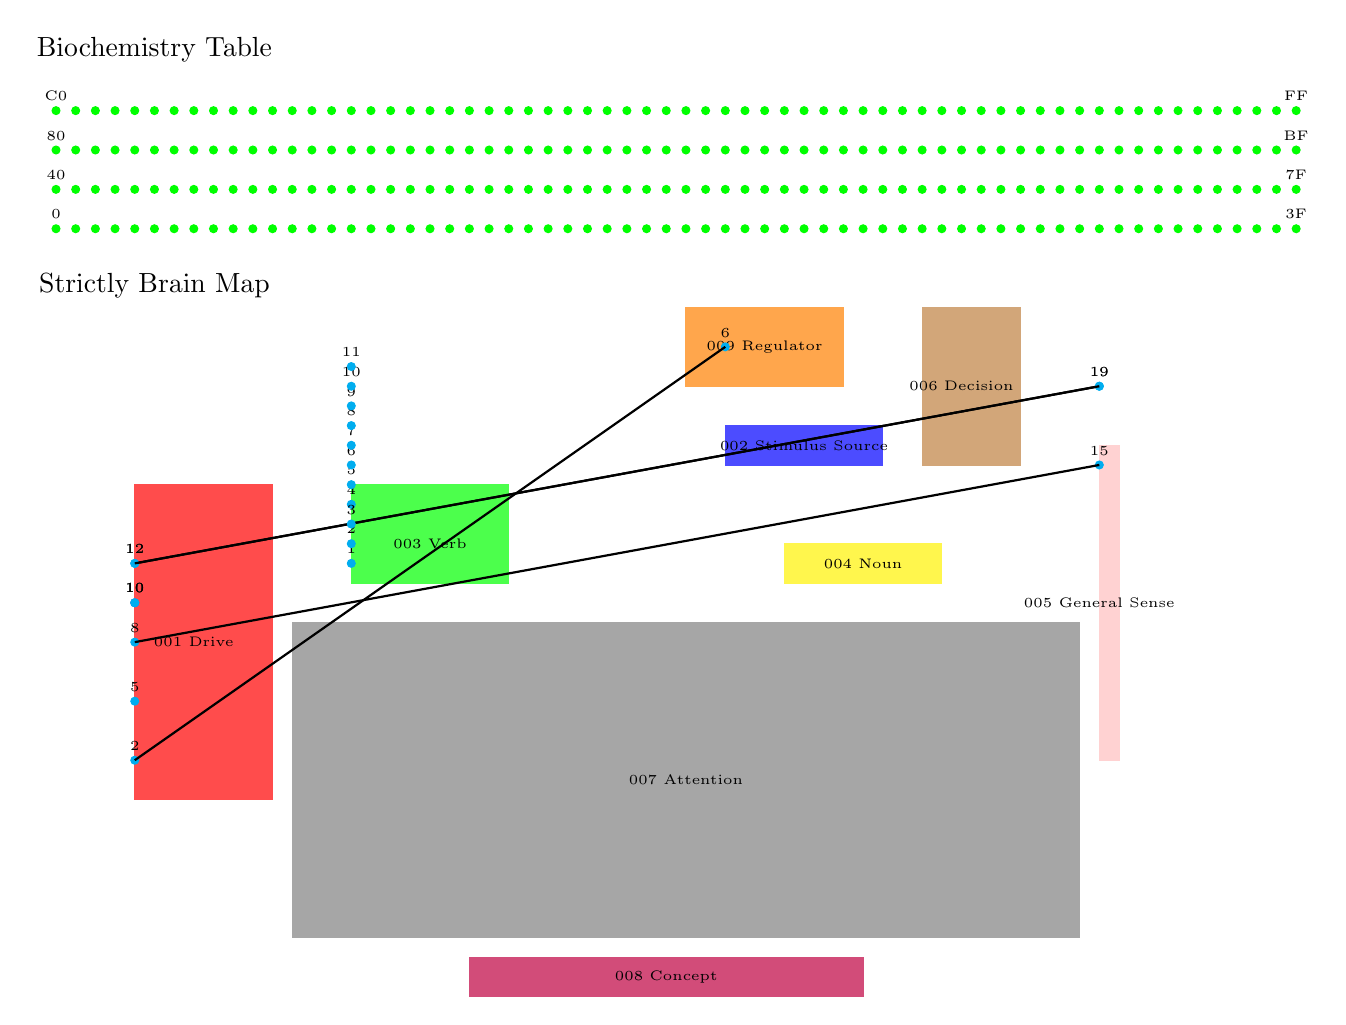
\begin{tikzpicture}[scale=0.25]
\filldraw[red!70] (4,13) rectangle (11,29);
\node at (7,21) {\tiny 001 Drive};
\filldraw[blue!70] (34,30) rectangle (42,32);
\node at (38,31) {\tiny 002 Stimulus Source};
\filldraw[green!70] (15,24) rectangle (23,29);
\node at (19,26) {\tiny 003 Verb};
\filldraw[yellow!70] (37,24) rectangle (45,26);
\node at (41,25) {\tiny 004 Noun};
\filldraw[purple!70] (21,3) rectangle (41,5);
\node at (31,4) {\tiny 008 Concept};
\filldraw[orange!70] (32,34) rectangle (40,38);
\node at (36,36) {\tiny 009 Regulator};
\filldraw[pink!70] (53,15) rectangle (54,31);
\node at (53,23) {\tiny 005 General Sense};
\filldraw[brown!70] (44,30) rectangle (49,38);
\node at (46,34) {\tiny 006 Decision};
\filldraw[gray!70] (12,6) rectangle (52,22);
\node at (32,14) {\tiny 007 Attention};
\filldraw[cyan] (15,25) circle (0.2);
\node at (15,25) [above, font=\tiny] {1};
\filldraw[cyan] (15,26) circle (0.2);
\node at (15,26) [above, font=\tiny] {2};
\filldraw[cyan] (15,28) circle (0.2);
\node at (15,28) [above, font=\tiny] {4};
\filldraw[magenta] (4,23) circle (0.2);
\node at (4,23) [above, font=\tiny] {10};
\filldraw[cyan] (4,18) circle (0.2);
\node at (4,18) [above, font=\tiny] {5};
\filldraw[cyan] (4,23) circle (0.2);
\node at (4,23) [above, font=\tiny] {10};
\filldraw[cyan] (4,23) circle (0.2);
\node at (4,23) [above, font=\tiny] {10};
\filldraw[cyan] (4,25) circle (0.2);
\node at (4,25) [above, font=\tiny] {12};
\filldraw[cyan] (53,34) circle (0.2);
\node at (53,34) [above, font=\tiny] {19};
\draw[thick, black] (53,34) -- (4,25) ;
\filldraw[cyan] (4,25) circle (0.2);
\node at (4,25) [above, font=\tiny] {12};
\filldraw[cyan] (53,34) circle (0.2);
\node at (53,34) [above, font=\tiny] {19};
\draw[thick, black] (53,34) -- (4,25) ;
\filldraw[cyan] (15,27) circle (0.2);
\node at (15,27) [above, font=\tiny] {3};
\filldraw[cyan] (15,29) circle (0.2);
\node at (15,29) [above, font=\tiny] {5};
\filldraw[cyan] (15,30) circle (0.2);
\node at (15,30) [above, font=\tiny] {6};
\filldraw[cyan] (15,31) circle (0.2);
\node at (15,31) [above, font=\tiny] {7};
\filldraw[cyan] (15,32) circle (0.2);
\node at (15,32) [above, font=\tiny] {8};
\filldraw[cyan] (15,33) circle (0.2);
\node at (15,33) [above, font=\tiny] {9};
\filldraw[cyan] (15,34) circle (0.2);
\node at (15,34) [above, font=\tiny] {10};
\filldraw[cyan] (15,35) circle (0.2);
\node at (15,35) [above, font=\tiny] {11};
\filldraw[cyan] (4,21) circle (0.2);
\node at (4,21) [above, font=\tiny] {8};
\filldraw[cyan] (53,30) circle (0.2);
\node at (53,30) [above, font=\tiny] {15};
\draw[thick, black] (53,30) -- (4,21) ;
\filldraw[cyan] (34,36) circle (0.2);
\node at (34,36) [above, font=\tiny] {6};
\filldraw[cyan] (4,15) circle (0.2);
\node at (4,15) [above, font=\tiny] {2};
\draw[thick, black] (4,15) -- (34,36) ;
\node at (5,50) [above] {Biochemistry Table};
\node at (5,38) [above] {Strictly Brain Map};
\filldraw[green] (0,42) circle (0.2);
\node at (0,42) [above, font=\tiny] {0};
\filldraw[green] (1,42) circle (0.2);
\node at (1,42) [above, font=\tiny] {};
\filldraw[green] (2,42) circle (0.2);
\node at (2,42) [above, font=\tiny] {};
\filldraw[green] (3,42) circle (0.2);
\node at (3,42) [above, font=\tiny] {};
\filldraw[green] (4,42) circle (0.2);
\node at (4,42) [above, font=\tiny] {};
\filldraw[green] (5,42) circle (0.2);
\node at (5,42) [above, font=\tiny] {};
\filldraw[green] (6,42) circle (0.2);
\node at (6,42) [above, font=\tiny] {};
\filldraw[green] (7,42) circle (0.2);
\node at (7,42) [above, font=\tiny] {};
\filldraw[green] (8,42) circle (0.2);
\node at (8,42) [above, font=\tiny] {};
\filldraw[green] (9,42) circle (0.2);
\node at (9,42) [above, font=\tiny] {};
\filldraw[green] (10,42) circle (0.2);
\node at (10,42) [above, font=\tiny] {};
\filldraw[green] (11,42) circle (0.2);
\node at (11,42) [above, font=\tiny] {};
\filldraw[green] (12,42) circle (0.2);
\node at (12,42) [above, font=\tiny] {};
\filldraw[green] (13,42) circle (0.2);
\node at (13,42) [above, font=\tiny] {};
\filldraw[green] (14,42) circle (0.2);
\node at (14,42) [above, font=\tiny] {};
\filldraw[green] (15,42) circle (0.2);
\node at (15,42) [above, font=\tiny] {};
\filldraw[green] (16,42) circle (0.2);
\node at (16,42) [above, font=\tiny] {};
\filldraw[green] (17,42) circle (0.2);
\node at (17,42) [above, font=\tiny] {};
\filldraw[green] (18,42) circle (0.2);
\node at (18,42) [above, font=\tiny] {};
\filldraw[green] (19,42) circle (0.2);
\node at (19,42) [above, font=\tiny] {};
\filldraw[green] (20,42) circle (0.2);
\node at (20,42) [above, font=\tiny] {};
\filldraw[green] (21,42) circle (0.2);
\node at (21,42) [above, font=\tiny] {};
\filldraw[green] (22,42) circle (0.2);
\node at (22,42) [above, font=\tiny] {};
\filldraw[green] (23,42) circle (0.2);
\node at (23,42) [above, font=\tiny] {};
\filldraw[green] (24,42) circle (0.2);
\node at (24,42) [above, font=\tiny] {};
\filldraw[green] (25,42) circle (0.2);
\node at (25,42) [above, font=\tiny] {};
\filldraw[green] (26,42) circle (0.2);
\node at (26,42) [above, font=\tiny] {};
\filldraw[green] (27,42) circle (0.2);
\node at (27,42) [above, font=\tiny] {};
\filldraw[green] (28,42) circle (0.2);
\node at (28,42) [above, font=\tiny] {};
\filldraw[green] (29,42) circle (0.2);
\node at (29,42) [above, font=\tiny] {};
\filldraw[green] (30,42) circle (0.2);
\node at (30,42) [above, font=\tiny] {};
\filldraw[green] (31,42) circle (0.2);
\node at (31,42) [above, font=\tiny] {};
\filldraw[green] (32,42) circle (0.2);
\node at (32,42) [above, font=\tiny] {};
\filldraw[green] (33,42) circle (0.2);
\node at (33,42) [above, font=\tiny] {};
\filldraw[green] (34,42) circle (0.2);
\node at (34,42) [above, font=\tiny] {};
\filldraw[green] (35,42) circle (0.2);
\node at (35,42) [above, font=\tiny] {};
\filldraw[green] (36,42) circle (0.2);
\node at (36,42) [above, font=\tiny] {};
\filldraw[green] (37,42) circle (0.2);
\node at (37,42) [above, font=\tiny] {};
\filldraw[green] (38,42) circle (0.2);
\node at (38,42) [above, font=\tiny] {};
\filldraw[green] (39,42) circle (0.2);
\node at (39,42) [above, font=\tiny] {};
\filldraw[green] (40,42) circle (0.2);
\node at (40,42) [above, font=\tiny] {};
\filldraw[green] (41,42) circle (0.2);
\node at (41,42) [above, font=\tiny] {};
\filldraw[green] (42,42) circle (0.2);
\node at (42,42) [above, font=\tiny] {};
\filldraw[green] (43,42) circle (0.2);
\node at (43,42) [above, font=\tiny] {};
\filldraw[green] (44,42) circle (0.2);
\node at (44,42) [above, font=\tiny] {};
\filldraw[green] (45,42) circle (0.2);
\node at (45,42) [above, font=\tiny] {};
\filldraw[green] (46,42) circle (0.2);
\node at (46,42) [above, font=\tiny] {};
\filldraw[green] (47,42) circle (0.2);
\node at (47,42) [above, font=\tiny] {};
\filldraw[green] (48,42) circle (0.2);
\node at (48,42) [above, font=\tiny] {};
\filldraw[green] (49,42) circle (0.2);
\node at (49,42) [above, font=\tiny] {};
\filldraw[green] (50,42) circle (0.2);
\node at (50,42) [above, font=\tiny] {};
\filldraw[green] (51,42) circle (0.2);
\node at (51,42) [above, font=\tiny] {};
\filldraw[green] (52,42) circle (0.2);
\node at (52,42) [above, font=\tiny] {};
\filldraw[green] (53,42) circle (0.2);
\node at (53,42) [above, font=\tiny] {};
\filldraw[green] (54,42) circle (0.2);
\node at (54,42) [above, font=\tiny] {};
\filldraw[green] (55,42) circle (0.2);
\node at (55,42) [above, font=\tiny] {};
\filldraw[green] (56,42) circle (0.2);
\node at (56,42) [above, font=\tiny] {};
\filldraw[green] (57,42) circle (0.2);
\node at (57,42) [above, font=\tiny] {};
\filldraw[green] (58,42) circle (0.2);
\node at (58,42) [above, font=\tiny] {};
\filldraw[green] (59,42) circle (0.2);
\node at (59,42) [above, font=\tiny] {};
\filldraw[green] (60,42) circle (0.2);
\node at (60,42) [above, font=\tiny] {};
\filldraw[green] (61,42) circle (0.2);
\node at (61,42) [above, font=\tiny] {};
\filldraw[green] (62,42) circle (0.2);
\node at (62,42) [above, font=\tiny] {};
\filldraw[green] (63,42) circle (0.2);
\node at (63,42) [above, font=\tiny] {3F};
\filldraw[green] (0,44) circle (0.2);
\node at (0,44) [above, font=\tiny] {40};
\filldraw[green] (1,44) circle (0.2);
\node at (1,44) [above, font=\tiny] {};
\filldraw[green] (2,44) circle (0.2);
\node at (2,44) [above, font=\tiny] {};
\filldraw[green] (3,44) circle (0.2);
\node at (3,44) [above, font=\tiny] {};
\filldraw[green] (4,44) circle (0.2);
\node at (4,44) [above, font=\tiny] {};
\filldraw[green] (5,44) circle (0.2);
\node at (5,44) [above, font=\tiny] {};
\filldraw[green] (6,44) circle (0.2);
\node at (6,44) [above, font=\tiny] {};
\filldraw[green] (7,44) circle (0.2);
\node at (7,44) [above, font=\tiny] {};
\filldraw[green] (8,44) circle (0.2);
\node at (8,44) [above, font=\tiny] {};
\filldraw[green] (9,44) circle (0.2);
\node at (9,44) [above, font=\tiny] {};
\filldraw[green] (10,44) circle (0.2);
\node at (10,44) [above, font=\tiny] {};
\filldraw[green] (11,44) circle (0.2);
\node at (11,44) [above, font=\tiny] {};
\filldraw[green] (12,44) circle (0.2);
\node at (12,44) [above, font=\tiny] {};
\filldraw[green] (13,44) circle (0.2);
\node at (13,44) [above, font=\tiny] {};
\filldraw[green] (14,44) circle (0.2);
\node at (14,44) [above, font=\tiny] {};
\filldraw[green] (15,44) circle (0.2);
\node at (15,44) [above, font=\tiny] {};
\filldraw[green] (16,44) circle (0.2);
\node at (16,44) [above, font=\tiny] {};
\filldraw[green] (17,44) circle (0.2);
\node at (17,44) [above, font=\tiny] {};
\filldraw[green] (18,44) circle (0.2);
\node at (18,44) [above, font=\tiny] {};
\filldraw[green] (19,44) circle (0.2);
\node at (19,44) [above, font=\tiny] {};
\filldraw[green] (20,44) circle (0.2);
\node at (20,44) [above, font=\tiny] {};
\filldraw[green] (21,44) circle (0.2);
\node at (21,44) [above, font=\tiny] {};
\filldraw[green] (22,44) circle (0.2);
\node at (22,44) [above, font=\tiny] {};
\filldraw[green] (23,44) circle (0.2);
\node at (23,44) [above, font=\tiny] {};
\filldraw[green] (24,44) circle (0.2);
\node at (24,44) [above, font=\tiny] {};
\filldraw[green] (25,44) circle (0.2);
\node at (25,44) [above, font=\tiny] {};
\filldraw[green] (26,44) circle (0.2);
\node at (26,44) [above, font=\tiny] {};
\filldraw[green] (27,44) circle (0.2);
\node at (27,44) [above, font=\tiny] {};
\filldraw[green] (28,44) circle (0.2);
\node at (28,44) [above, font=\tiny] {};
\filldraw[green] (29,44) circle (0.2);
\node at (29,44) [above, font=\tiny] {};
\filldraw[green] (30,44) circle (0.2);
\node at (30,44) [above, font=\tiny] {};
\filldraw[green] (31,44) circle (0.2);
\node at (31,44) [above, font=\tiny] {};
\filldraw[green] (32,44) circle (0.2);
\node at (32,44) [above, font=\tiny] {};
\filldraw[green] (33,44) circle (0.2);
\node at (33,44) [above, font=\tiny] {};
\filldraw[green] (34,44) circle (0.2);
\node at (34,44) [above, font=\tiny] {};
\filldraw[green] (35,44) circle (0.2);
\node at (35,44) [above, font=\tiny] {};
\filldraw[green] (36,44) circle (0.2);
\node at (36,44) [above, font=\tiny] {};
\filldraw[green] (37,44) circle (0.2);
\node at (37,44) [above, font=\tiny] {};
\filldraw[green] (38,44) circle (0.2);
\node at (38,44) [above, font=\tiny] {};
\filldraw[green] (39,44) circle (0.2);
\node at (39,44) [above, font=\tiny] {};
\filldraw[green] (40,44) circle (0.2);
\node at (40,44) [above, font=\tiny] {};
\filldraw[green] (41,44) circle (0.2);
\node at (41,44) [above, font=\tiny] {};
\filldraw[green] (42,44) circle (0.2);
\node at (42,44) [above, font=\tiny] {};
\filldraw[green] (43,44) circle (0.2);
\node at (43,44) [above, font=\tiny] {};
\filldraw[green] (44,44) circle (0.2);
\node at (44,44) [above, font=\tiny] {};
\filldraw[green] (45,44) circle (0.2);
\node at (45,44) [above, font=\tiny] {};
\filldraw[green] (46,44) circle (0.2);
\node at (46,44) [above, font=\tiny] {};
\filldraw[green] (47,44) circle (0.2);
\node at (47,44) [above, font=\tiny] {};
\filldraw[green] (48,44) circle (0.2);
\node at (48,44) [above, font=\tiny] {};
\filldraw[green] (49,44) circle (0.2);
\node at (49,44) [above, font=\tiny] {};
\filldraw[green] (50,44) circle (0.2);
\node at (50,44) [above, font=\tiny] {};
\filldraw[green] (51,44) circle (0.2);
\node at (51,44) [above, font=\tiny] {};
\filldraw[green] (52,44) circle (0.2);
\node at (52,44) [above, font=\tiny] {};
\filldraw[green] (53,44) circle (0.2);
\node at (53,44) [above, font=\tiny] {};
\filldraw[green] (54,44) circle (0.2);
\node at (54,44) [above, font=\tiny] {};
\filldraw[green] (55,44) circle (0.2);
\node at (55,44) [above, font=\tiny] {};
\filldraw[green] (56,44) circle (0.2);
\node at (56,44) [above, font=\tiny] {};
\filldraw[green] (57,44) circle (0.2);
\node at (57,44) [above, font=\tiny] {};
\filldraw[green] (58,44) circle (0.2);
\node at (58,44) [above, font=\tiny] {};
\filldraw[green] (59,44) circle (0.2);
\node at (59,44) [above, font=\tiny] {};
\filldraw[green] (60,44) circle (0.2);
\node at (60,44) [above, font=\tiny] {};
\filldraw[green] (61,44) circle (0.2);
\node at (61,44) [above, font=\tiny] {};
\filldraw[green] (62,44) circle (0.2);
\node at (62,44) [above, font=\tiny] {};
\filldraw[green] (63,44) circle (0.2);
\node at (63,44) [above, font=\tiny] {7F};
\filldraw[green] (0,46) circle (0.2);
\node at (0,46) [above, font=\tiny] {80};
\filldraw[green] (1,46) circle (0.2);
\node at (1,46) [above, font=\tiny] {};
\filldraw[green] (2,46) circle (0.2);
\node at (2,46) [above, font=\tiny] {};
\filldraw[green] (3,46) circle (0.2);
\node at (3,46) [above, font=\tiny] {};
\filldraw[green] (4,46) circle (0.2);
\node at (4,46) [above, font=\tiny] {};
\filldraw[green] (5,46) circle (0.2);
\node at (5,46) [above, font=\tiny] {};
\filldraw[green] (6,46) circle (0.2);
\node at (6,46) [above, font=\tiny] {};
\filldraw[green] (7,46) circle (0.2);
\node at (7,46) [above, font=\tiny] {};
\filldraw[green] (8,46) circle (0.2);
\node at (8,46) [above, font=\tiny] {};
\filldraw[green] (9,46) circle (0.2);
\node at (9,46) [above, font=\tiny] {};
\filldraw[green] (10,46) circle (0.2);
\node at (10,46) [above, font=\tiny] {};
\filldraw[green] (11,46) circle (0.2);
\node at (11,46) [above, font=\tiny] {};
\filldraw[green] (12,46) circle (0.2);
\node at (12,46) [above, font=\tiny] {};
\filldraw[green] (13,46) circle (0.2);
\node at (13,46) [above, font=\tiny] {};
\filldraw[green] (14,46) circle (0.2);
\node at (14,46) [above, font=\tiny] {};
\filldraw[green] (15,46) circle (0.2);
\node at (15,46) [above, font=\tiny] {};
\filldraw[green] (16,46) circle (0.2);
\node at (16,46) [above, font=\tiny] {};
\filldraw[green] (17,46) circle (0.2);
\node at (17,46) [above, font=\tiny] {};
\filldraw[green] (18,46) circle (0.2);
\node at (18,46) [above, font=\tiny] {};
\filldraw[green] (19,46) circle (0.2);
\node at (19,46) [above, font=\tiny] {};
\filldraw[green] (20,46) circle (0.2);
\node at (20,46) [above, font=\tiny] {};
\filldraw[green] (21,46) circle (0.2);
\node at (21,46) [above, font=\tiny] {};
\filldraw[green] (22,46) circle (0.2);
\node at (22,46) [above, font=\tiny] {};
\filldraw[green] (23,46) circle (0.2);
\node at (23,46) [above, font=\tiny] {};
\filldraw[green] (24,46) circle (0.2);
\node at (24,46) [above, font=\tiny] {};
\filldraw[green] (25,46) circle (0.2);
\node at (25,46) [above, font=\tiny] {};
\filldraw[green] (26,46) circle (0.2);
\node at (26,46) [above, font=\tiny] {};
\filldraw[green] (27,46) circle (0.2);
\node at (27,46) [above, font=\tiny] {};
\filldraw[green] (28,46) circle (0.2);
\node at (28,46) [above, font=\tiny] {};
\filldraw[green] (29,46) circle (0.2);
\node at (29,46) [above, font=\tiny] {};
\filldraw[green] (30,46) circle (0.2);
\node at (30,46) [above, font=\tiny] {};
\filldraw[green] (31,46) circle (0.2);
\node at (31,46) [above, font=\tiny] {};
\filldraw[green] (32,46) circle (0.2);
\node at (32,46) [above, font=\tiny] {};
\filldraw[green] (33,46) circle (0.2);
\node at (33,46) [above, font=\tiny] {};
\filldraw[green] (34,46) circle (0.2);
\node at (34,46) [above, font=\tiny] {};
\filldraw[green] (35,46) circle (0.2);
\node at (35,46) [above, font=\tiny] {};
\filldraw[green] (36,46) circle (0.2);
\node at (36,46) [above, font=\tiny] {};
\filldraw[green] (37,46) circle (0.2);
\node at (37,46) [above, font=\tiny] {};
\filldraw[green] (38,46) circle (0.2);
\node at (38,46) [above, font=\tiny] {};
\filldraw[green] (39,46) circle (0.2);
\node at (39,46) [above, font=\tiny] {};
\filldraw[green] (40,46) circle (0.2);
\node at (40,46) [above, font=\tiny] {};
\filldraw[green] (41,46) circle (0.2);
\node at (41,46) [above, font=\tiny] {};
\filldraw[green] (42,46) circle (0.2);
\node at (42,46) [above, font=\tiny] {};
\filldraw[green] (43,46) circle (0.2);
\node at (43,46) [above, font=\tiny] {};
\filldraw[green] (44,46) circle (0.2);
\node at (44,46) [above, font=\tiny] {};
\filldraw[green] (45,46) circle (0.2);
\node at (45,46) [above, font=\tiny] {};
\filldraw[green] (46,46) circle (0.2);
\node at (46,46) [above, font=\tiny] {};
\filldraw[green] (47,46) circle (0.2);
\node at (47,46) [above, font=\tiny] {};
\filldraw[green] (48,46) circle (0.2);
\node at (48,46) [above, font=\tiny] {};
\filldraw[green] (49,46) circle (0.2);
\node at (49,46) [above, font=\tiny] {};
\filldraw[green] (50,46) circle (0.2);
\node at (50,46) [above, font=\tiny] {};
\filldraw[green] (51,46) circle (0.2);
\node at (51,46) [above, font=\tiny] {};
\filldraw[green] (52,46) circle (0.2);
\node at (52,46) [above, font=\tiny] {};
\filldraw[green] (53,46) circle (0.2);
\node at (53,46) [above, font=\tiny] {};
\filldraw[green] (54,46) circle (0.2);
\node at (54,46) [above, font=\tiny] {};
\filldraw[green] (55,46) circle (0.2);
\node at (55,46) [above, font=\tiny] {};
\filldraw[green] (56,46) circle (0.2);
\node at (56,46) [above, font=\tiny] {};
\filldraw[green] (57,46) circle (0.2);
\node at (57,46) [above, font=\tiny] {};
\filldraw[green] (58,46) circle (0.2);
\node at (58,46) [above, font=\tiny] {};
\filldraw[green] (59,46) circle (0.2);
\node at (59,46) [above, font=\tiny] {};
\filldraw[green] (60,46) circle (0.2);
\node at (60,46) [above, font=\tiny] {};
\filldraw[green] (61,46) circle (0.2);
\node at (61,46) [above, font=\tiny] {};
\filldraw[green] (62,46) circle (0.2);
\node at (62,46) [above, font=\tiny] {};
\filldraw[green] (63,46) circle (0.2);
\node at (63,46) [above, font=\tiny] {BF};
\filldraw[green] (0,48) circle (0.2);
\node at (0,48) [above, font=\tiny] {C0};
\filldraw[green] (1,48) circle (0.2);
\node at (1,48) [above, font=\tiny] {};
\filldraw[green] (2,48) circle (0.2);
\node at (2,48) [above, font=\tiny] {};
\filldraw[green] (3,48) circle (0.2);
\node at (3,48) [above, font=\tiny] {};
\filldraw[green] (4,48) circle (0.2);
\node at (4,48) [above, font=\tiny] {};
\filldraw[green] (5,48) circle (0.2);
\node at (5,48) [above, font=\tiny] {};
\filldraw[green] (6,48) circle (0.2);
\node at (6,48) [above, font=\tiny] {};
\filldraw[green] (7,48) circle (0.2);
\node at (7,48) [above, font=\tiny] {};
\filldraw[green] (8,48) circle (0.2);
\node at (8,48) [above, font=\tiny] {};
\filldraw[green] (9,48) circle (0.2);
\node at (9,48) [above, font=\tiny] {};
\filldraw[green] (10,48) circle (0.2);
\node at (10,48) [above, font=\tiny] {};
\filldraw[green] (11,48) circle (0.2);
\node at (11,48) [above, font=\tiny] {};
\filldraw[green] (12,48) circle (0.2);
\node at (12,48) [above, font=\tiny] {};
\filldraw[green] (13,48) circle (0.2);
\node at (13,48) [above, font=\tiny] {};
\filldraw[green] (14,48) circle (0.2);
\node at (14,48) [above, font=\tiny] {};
\filldraw[green] (15,48) circle (0.2);
\node at (15,48) [above, font=\tiny] {};
\filldraw[green] (16,48) circle (0.2);
\node at (16,48) [above, font=\tiny] {};
\filldraw[green] (17,48) circle (0.2);
\node at (17,48) [above, font=\tiny] {};
\filldraw[green] (18,48) circle (0.2);
\node at (18,48) [above, font=\tiny] {};
\filldraw[green] (19,48) circle (0.2);
\node at (19,48) [above, font=\tiny] {};
\filldraw[green] (20,48) circle (0.2);
\node at (20,48) [above, font=\tiny] {};
\filldraw[green] (21,48) circle (0.2);
\node at (21,48) [above, font=\tiny] {};
\filldraw[green] (22,48) circle (0.2);
\node at (22,48) [above, font=\tiny] {};
\filldraw[green] (23,48) circle (0.2);
\node at (23,48) [above, font=\tiny] {};
\filldraw[green] (24,48) circle (0.2);
\node at (24,48) [above, font=\tiny] {};
\filldraw[green] (25,48) circle (0.2);
\node at (25,48) [above, font=\tiny] {};
\filldraw[green] (26,48) circle (0.2);
\node at (26,48) [above, font=\tiny] {};
\filldraw[green] (27,48) circle (0.2);
\node at (27,48) [above, font=\tiny] {};
\filldraw[green] (28,48) circle (0.2);
\node at (28,48) [above, font=\tiny] {};
\filldraw[green] (29,48) circle (0.2);
\node at (29,48) [above, font=\tiny] {};
\filldraw[green] (30,48) circle (0.2);
\node at (30,48) [above, font=\tiny] {};
\filldraw[green] (31,48) circle (0.2);
\node at (31,48) [above, font=\tiny] {};
\filldraw[green] (32,48) circle (0.2);
\node at (32,48) [above, font=\tiny] {};
\filldraw[green] (33,48) circle (0.2);
\node at (33,48) [above, font=\tiny] {};
\filldraw[green] (34,48) circle (0.2);
\node at (34,48) [above, font=\tiny] {};
\filldraw[green] (35,48) circle (0.2);
\node at (35,48) [above, font=\tiny] {};
\filldraw[green] (36,48) circle (0.2);
\node at (36,48) [above, font=\tiny] {};
\filldraw[green] (37,48) circle (0.2);
\node at (37,48) [above, font=\tiny] {};
\filldraw[green] (38,48) circle (0.2);
\node at (38,48) [above, font=\tiny] {};
\filldraw[green] (39,48) circle (0.2);
\node at (39,48) [above, font=\tiny] {};
\filldraw[green] (40,48) circle (0.2);
\node at (40,48) [above, font=\tiny] {};
\filldraw[green] (41,48) circle (0.2);
\node at (41,48) [above, font=\tiny] {};
\filldraw[green] (42,48) circle (0.2);
\node at (42,48) [above, font=\tiny] {};
\filldraw[green] (43,48) circle (0.2);
\node at (43,48) [above, font=\tiny] {};
\filldraw[green] (44,48) circle (0.2);
\node at (44,48) [above, font=\tiny] {};
\filldraw[green] (45,48) circle (0.2);
\node at (45,48) [above, font=\tiny] {};
\filldraw[green] (46,48) circle (0.2);
\node at (46,48) [above, font=\tiny] {};
\filldraw[green] (47,48) circle (0.2);
\node at (47,48) [above, font=\tiny] {};
\filldraw[green] (48,48) circle (0.2);
\node at (48,48) [above, font=\tiny] {};
\filldraw[green] (49,48) circle (0.2);
\node at (49,48) [above, font=\tiny] {};
\filldraw[green] (50,48) circle (0.2);
\node at (50,48) [above, font=\tiny] {};
\filldraw[green] (51,48) circle (0.2);
\node at (51,48) [above, font=\tiny] {};
\filldraw[green] (52,48) circle (0.2);
\node at (52,48) [above, font=\tiny] {};
\filldraw[green] (53,48) circle (0.2);
\node at (53,48) [above, font=\tiny] {};
\filldraw[green] (54,48) circle (0.2);
\node at (54,48) [above, font=\tiny] {};
\filldraw[green] (55,48) circle (0.2);
\node at (55,48) [above, font=\tiny] {};
\filldraw[green] (56,48) circle (0.2);
\node at (56,48) [above, font=\tiny] {};
\filldraw[green] (57,48) circle (0.2);
\node at (57,48) [above, font=\tiny] {};
\filldraw[green] (58,48) circle (0.2);
\node at (58,48) [above, font=\tiny] {};
\filldraw[green] (59,48) circle (0.2);
\node at (59,48) [above, font=\tiny] {};
\filldraw[green] (60,48) circle (0.2);
\node at (60,48) [above, font=\tiny] {};
\filldraw[green] (61,48) circle (0.2);
\node at (61,48) [above, font=\tiny] {};
\filldraw[green] (62,48) circle (0.2);
\node at (62,48) [above, font=\tiny] {};
\filldraw[green] (63,48) circle (0.2);
\node at (63,48) [above, font=\tiny] {FF};
\end{tikzpicture}
\end{center}

\newpage

\section*{Instincts}

Number :19

\begin{longtable}{|p{3cm}|p{3cm}|p{3cm}|p{8cm}|}
\hline
{\bf Action} & {\bf Reinforcement Drive} & {\bf Reinforcement Level} & {\bf Conditions} \\ \hline
Activate 1 (push) it & Reward & 255 & Verb (3)[1/Activate 1 it]~\newline  \\ \hline
Activate 2 (pull) it & Reward & 255 & Verb (3)[2/Activate 2 it]~\newline  \\ \hline
Approach it & Reward & 255 & Verb (3)[4/Approach it]~\newline  \\ \hline
Move & Punish & 255 & Drive (1)[10/Boredom]~\newline  \\ \hline
Rest & Reward & 93 & Drive (1)[5/Tiredness]~\newline  \\ \hline
Activate 1 (push) it & Reward & 255 & Drive (1)[10/Boredom]~\newline  \\ \hline
Activate 2 (pull) it & Reward & 255 & Drive (1)[10/Boredom]~\newline  \\ \hline
Activate 1 (push) it & Reward & 255 & Drive (1)[12/Sex drive]~\newline General Sense (5)[19/IT is opposite sex]~\newline  \\ \hline
Activate 2 (pull) it & Reward & 112 & Drive (1)[12/Sex drive]~\newline General Sense (5)[19/IT is opposite sex]~\newline  \\ \hline
Deactivate it & Reward & 255 & Verb (3)[3/Deactivate it]~\newline  \\ \hline
Retreat frm it & Reward & 255 & Verb (3)[5/Retreat frm it]~\newline  \\ \hline
Get it & Reward & 255 & Verb (3)[6/Get it]~\newline  \\ \hline
Drop all & Reward & 255 & Verb (3)[7/Drop all]~\newline  \\ \hline
Say what you need (how?) & Reward & 255 & Verb (3)[8/Say what you need]~\newline  \\ \hline
Rest & Reward & 255 & Verb (3)[9/Rest]~\newline  \\ \hline
Travel west & Reward & 255 & Verb (3)[10/Travel west]~\newline  \\ \hline
Travel east & Reward & 255 & Verb (3)[11/Travel east]~\newline  \\ \hline
Retreat frm it & Reward & 255 & Drive (1)[8/Crowded]~\newline General Sense (5)[15/IT is a creature]~\newline  \\ \hline
Activate 1 (push) it & Reward & 255 & Stimulus Source (2)[6/<ID 6> (egg)]~\newline Drive (1)[2/Hunger]~\newline  \\ \hline
\end{longtable}

\newpage

\section*{Receptors}

Number :43

\begin{longtable}{|p{7cm}|p{3cm}|p{2cm}|p{2cm}|p{2cm}|}
\hline
{\bf Locus} & {\bf Chemical} & {\bf Threshold} & {\bf Nominal} & {\bf Gain} \\ \hline
(Creature, Drive, Pain) & pain & 0 & 0 & 255 \\ \hline
(Creature, Drive, Need for pleasure) & need for pleasure & 0 & 0 & 255 \\ \hline
(Creature, Drive, Hunger) & hunger & 0 & 0 & 255 \\ \hline
(Creature, Drive, Coldness) & coldness & 0 & 0 & 255 \\ \hline
(Creature, Drive, Hotness) & hotness & 0 & 0 & 255 \\ \hline
(Creature, Drive, Tiredness) & tiredness & 0 & 0 & 255 \\ \hline
(Creature, Drive, Sleepiness) & sleepiness & 0 & 0 & 255 \\ \hline
(Creature, Drive, Loneliness) & loneliness & 0 & 0 & 255 \\ \hline
(Creature, Drive, Crowded) & crowded & 0 & 0 & 255 \\ \hline
(Creature, Drive, Fear) & fear & 0 & 0 & 255 \\ \hline
(Creature, Drive, Boredom) & boredom & 0 & 0 & 255 \\ \hline
(Creature, Drive, Anger) & anger & 0 & 0 & 255 \\ \hline
(Creature, Drive, Sex drive) & sex drive & 0 & 0 & 255 \\ \hline
(Brain, Decision o/ps, Chemical 0) & reward & 0 & 0 & 255 \\ \hline
(Brain, Decision o/ps, Chemical 1) & punishment & 0 & 0 & 255 \\ \hline
(Brain, Lobe 8, Chemical 1) & conASH & 0 & 4 & 255 \\ \hline
(Brain, Decision o/ps, Chemical 2) & decASH1 & 0 & 16 & 255 \\ \hline
(Brain, Decision o/ps, Chemical 3) & decASH2 & 0 & 16 & 255 \\ \hline
(Brain, Lobe 8, Chemical 0) & reinforcement & 0 & 0 & 255 \\ \hline
(Creature, Reproductive , Become fertile if high) & estrogen & 0 & 0 & 255 \\ \hline
(Creature, Reproductive , Receptive to sperm if > 0) & sex drive & 0 & 44 & 255 \\ \hline
(Creature, Sensorimotor, Involuntary action 1) & progesterone & 255 & 0 & 255 \\ \hline
(Creature, Reproductive , Become fertile if high) & testosterone & 0 & 0 & 255 \\ \hline
(Creature, Somatic, Become a child) & aging & 255 & 119 & 255 \\ \hline
(Creature, Somatic, Become youth) & aging & 255 & 116 & 255 \\ \hline
(Creature, Somatic, Become adolescent) & aging & 255 & 110 & 255 \\ \hline
(Creature, Somatic, Become adult) & aging & 120 & 120 & 255 \\ \hline
(Creature, Somatic, Become old) & aging & 76 & 119 & 255 \\ \hline
(Creature, Somatic, Become senile) & aging & 34 & 117 & 255 \\ \hline
(Creature, Immune, Die if non) & glycogen & 8 & 255 & 255 \\ \hline
(Creature, Sensorimotor, Involuntary action 0) & pain++ & 65 & 0 & 255 \\ \hline
(Creature, Sensorimotor, Involuntary action 2) & antigen 7 & 58 & 0 & 255 \\ \hline
(Creature, Sensorimotor, Involuntary action 3) & antigen 7 & 42 & 0 & 255 \\ \hline
(Creature, Sensorimotor, Involuntary action 4) & coldness & 255 & 0 & 255 \\ \hline
(Creature, Sensorimotor, Special gait 1) & pain & 48 & 0 & 255 \\ \hline
(Creature, Sensorimotor, Special gait 3) & fear & 255 & 0 & 255 \\ \hline
(Creature, Sensorimotor, Special gait 4) & anger & 255 & 0 & 255 \\ \hline
(Creature, Sensorimotor, Special gait 5) & sleepiness & 255 & 0 & 255 \\ \hline
(Creature, Sensorimotor, Special gait 6) & tiredness & 255 & 0 & 255 \\ \hline
(Creature, Sensorimotor, Special gait 2) & glycogen & 0 & 35 & 255 \\ \hline
(Creature, Sensorimotor, Special gait 7) & alcohol & 106 & 0 & 255 \\ \hline
(Creature, Sensorimotor, Involuntary action 5) & sleepiness & 255 & 0 & 255 \\ \hline
(Creature, Sensorimotor, Involuntary action 6) & glycogen & 20 & 127 & 255 \\ \hline
\end{longtable}

\newpage

\section*{Emitters}

Number :27

\begin{longtable}{|p{7cm}|p{3cm}|p{2cm}|p{2cm}|p{2cm}|}
\hline
{\bf Locus} & {\bf Chemical} & {\bf Threshold} & {\bf Sample Rate} & {\bf Gain} \\ \hline
(Brain, Lobe 8, \# Loose dens/cells type 0) & conASH & 0 & 1 & 255 \\ \hline
(Brain, Decision o/ps, \# Loose dens/cells type 0) & decASH1 & 0 & 1 & 255 \\ \hline
(Brain, Decision o/ps, \# Loose dens/cells type 1) & decASH2 & 0 & 1 & 255 \\ \hline
(Creature, Sensorimotor, I'm asleep (255)) & boredom & 0 & 25 & 8 \\ \hline
(Creature, Sensorimotor, I'm asleep (255)) & need for pleasure & 0 & 64 & 10 \\ \hline
(Creature, Sensorimotor, Air is this hot) & hotness & 0 & 24 & 49 \\ \hline
(Creature, Sensorimotor, Air is this cold) & coldness & 0 & 24 & 50 \\ \hline
(Creature, Sensorimotor, Light level) & sleepiness & 0 & 114 & 8 \\ \hline
(Creature, Sensorimotor, Crowdedness) & loneliness & 0 & 18 & 5 \\ \hline
(Creature, Sensorimotor, Crowdedness) & crowded & 0 & 75 & 51 \\ \hline
(Creature, Somatic, Muscle energy used) & hexokinase & 0 & 17 & 1 \\ \hline
(Creature, Reproductive, I am fertile (egg/sperm ready)) & estrogen & 0 & 17 & 6 \\ \hline
(Creature, Reproductive, I am fertile (egg/sperm ready)) & sex drive & 0 & 20 & 7 \\ \hline
(Creature, Reproductive, I am pregnant (egg\&sperm ready)) & gonadotropin & 0 & 40 & 64 \\ \hline
(Creature, Reproductive, I am pregnant (egg\&sperm ready)) & progesterone & 0 & 13 & 4 \\ \hline
(Creature, Sensorimotor, Permanently active (255)) & testosterone & 0 & 19 & 6 \\ \hline
(Creature, Reproductive, I am fertile (egg/sperm ready)) & sex drive & 0 & 25 & 8 \\ \hline
(Creature, Drive, Pain) & adrenaline & 255 & 18 & 10 \\ \hline
(Creature, Drive, Hunger) & adrenaline & 255 & 21 & 8 \\ \hline
(Creature, Drive, Loneliness) & adrenaline & 255 & 26 & 14 \\ \hline
(Creature, Drive, Crowded) & adrenaline & 255 & 16 & 16 \\ \hline
(Creature, Drive, Fear) & adrenaline & 255 & 9 & 26 \\ \hline
(Creature, Drive, Boredom) & adrenaline & 255 & 25 & 7 \\ \hline
(Creature, Drive, Anger) & adrenaline & 255 & 11 & 33 \\ \hline
(Creature, Reproductive, I am fertile (egg/sperm ready)) & none & 0 & 82 & 5 \\ \hline
(Creature, Sensorimotor, Permanently active (255)) & testosterone & 0 & 49 & 6 \\ \hline
(Creature, Sensorimotor, I'm asleep (255)) & boredom & 0 & 47 & 8 \\ \hline
\end{longtable}

\newpage

\section*{Stimuli}

Number :26

\begin{longtable}{|p{2cm}|p{2cm}|p{2cm}|p{2cm}|p{1.50cm}|p{1.50cm}|p{1.50cm}|p{1.50cm}|}
\hline
{\bf SeqNum} & {\bf Significance} & {\bf SensoryNeu} & {\bf Intensity} & {\bf Locus 1} & {\bf Locus 2} & {\bf Locus 3} & {\bf Locus 4} \\ \hline
1 & 0 & 255 & 0 & (27,16) & (18,16) & (28,16) & (0,0) \\ \hline
2 & 32 & 0 & 255 & (34,64) & (33,16) & (40,16) & (49,16) \\ \hline
3 & 80 & 0 & 255 & (34,48) & (40,16) & (25,16) & (29,8) \\ \hline
4 & 32 & 1 & 255 & (17,75) & (26,32) & (28,16) & (39,16) \\ \hline
5 & 255 & 1 & 255 & (17,80) & (26,32) & (28,16) & (39,16) \\ \hline
6 & 82 & 10 & 255 & (0,0) & (0,0) & (0,0) & (0,0) \\ \hline
7 & 36 & 11 & 255 & (0,0) & (0,0) & (0,0) & (0,0) \\ \hline
8 & 0 & 2 & 255 & (17,25) & (0,0) & (0,0) & (0,0) \\ \hline
9 & 255 & 255 & 0 & (0,0) & (0,0) & (0,0) & (0,0) \\ \hline
10 & 16 & 8 & 255 & (0,0) & (0,0) & (0,0) & (0,0) \\ \hline
11 & 16 & 5 & 255 & (43,32) & (40,16) & (0,0) & (0,0) \\ \hline
12 & 16 & 6 & 255 & (43,16) & (40,16) & (25,16) & (0,0) \\ \hline
13 & 0 & 255 & 0 & (27,8) & (0,0) & (0,0) & (0,0) \\ \hline
14 & 0 & 255 & 0 & (22,3) & (43,16) & (0,0) & (0,0) \\ \hline
15 & 0 & 255 & 0 & (22,3) & (43,16) & (0,0) & (0,0) \\ \hline
16 & 0 & 255 & 0 & (22,2) & (0,0) & (0,0) & (0,0) \\ \hline
17 & 0 & 255 & 0 & (22,2) & (40,8) & (25,8) & (0,0) \\ \hline
18 & 0 & 255 & 0 & (22,3) & (40,16) & (0,0) & (0,0) \\ \hline
19 & 0 & 255 & 0 & (38,50) & (23,16) & (27,16) & (0,0) \\ \hline
20 & 0 & 255 & 0 & (38,66) & (39,77) & (27,16) & (20,16) \\ \hline
21 & 0 & 255 & 0 & (22,8) & (43,16) & (7,16) & (0,0) \\ \hline
22 & 0 & 255 & 0 & (1,255) & (6,255) & (7,112) & (61,32) \\ \hline
23 & 0 & 255 & 0 & (1,32) & (6,8) & (10,8) & (61,16) \\ \hline
24 & 0 & 255 & 0 & (1,32) & (6,8) & (10,8) & (61,16) \\ \hline
25 & 0 & 255 & 0 & (21,16) & (36,32) & (6,16) & (10,16) \\ \hline
26 & 0 & 255 & 0 & (22,22) & (43,16) & (7,32) & (0,0) \\ \hline
\end{longtable}

\newpage

\section*{Chemical Reactions}

Number :59

\begin{longtable}{|p{7cm}|p{7cm}|p{2cm}|}
\hline
{\bf Reactants} & {\bf Products} & {\bf Rate} \\ \hline
1*pain++ + 1*none & 1*pain + 1*punishment & 8 \\ \hline
1*need for pleasure++ + 1*none & 1*need for pleasure + 1*punishment & 8 \\ \hline
1*hunger++ + 1*none & 1*hunger + 1*punishment & 8 \\ \hline
1*coldness++ + 1*none & 1*coldness + 1*punishment & 8 \\ \hline
1*hotness++ + 1*none & 1*hotness + 1*punishment & 8 \\ \hline
1*tiredness++ + 1*none & 1*tiredness + 1*punishment & 8 \\ \hline
1*sleepiness++ + 1*none & 1*sleepiness + 1*punishment & 8 \\ \hline
1*loneliness++ + 1*none & 1*loneliness + 1*punishment & 8 \\ \hline
1*crowded++ + 1*none & 1*crowded + 1*punishment & 8 \\ \hline
1*fear++ + 1*none & 1*fear + 1*punishment & 8 \\ \hline
1*boredom++ + 1*none & 1*boredom + 1*punishment & 8 \\ \hline
1*anger++ + 1*none & 1*anger + 1*punishment & 8 \\ \hline
1*sex drive++ + 1*none & 1*sex drive + 1*punishment & 8 \\ \hline
1*pain-- + 1*pain & 1*reward + 1*none & 8 \\ \hline
1*need for pleasure-- + 1*need for pleasure & 1*reward + 1*none & 8 \\ \hline
1*hunger-- + 1*hunger & 1*reward + 1*none & 8 \\ \hline
1*coldness-- + 1*coldness & 1*reward + 1*none & 8 \\ \hline
1*hotness-- + 1*hotness & 1*reward + 1*none & 8 \\ \hline
1*tiredness-- + 1*tiredness & 1*reward + 1*none & 8 \\ \hline
1*sleepiness-- + 1*sleepiness & 1*reward + 1*none & 8 \\ \hline
1*loneliness-- + 1*loneliness & 1*reward + 1*none & 8 \\ \hline
1*crowded-- + 1*crowded & 1*reward + 1*none & 8 \\ \hline
1*fear-- + 1*fear & 1*reward + 1*none & 8 \\ \hline
1*boredom-- + 1*boredom & 1*reward + 1*none & 8 \\ \hline
1*anger-- + 1*anger & 1*reward + 1*none & 8 \\ \hline
1*sex drive-- + 1*sex drive & 1*reward + 1*none & 8 \\ \hline
1*reward + 1*none & 1*reinforcement + 1*rewardecho & 16 \\ \hline
1*punishment + 1*none & 1*reinforcement + 1*punishecho & 16 \\ \hline
1*starch + 1*none & 2*glucose + 1*none & 64 \\ \hline
3*glucose + 1*none & 1*glycogen + 1*hunger-- & 56 \\ \hline
1*glycogen + 1*none & 3*glucose + 1*hunger & 64 \\ \hline
1*glucose + 2*hexokinase & 4*CO2 + 1*none & 24 \\ \hline
1*gonadotropin + 2*estrogen & 1*gonadotropin + 1*none & 40 \\ \hline
1*glycotoxin + 2*glycogen & 2*pain++ + 2*sleepiness++ & 72 \\ \hline
2*antigen 7 + 4*glucose & 1*antigen 7 + 1*hotness & 88 \\ \hline
2*antigen 7 + 4*glucose & 1*antigen 7 + 1*hotness & 88 \\ \hline
2*antigen 7 + 4*glucose & 1*antigen 7 + 1*hotness & 88 \\ \hline
2*antigen 7 + 4*glucose & 1*antigen 7 + 1*hotness & 80 \\ \hline
2*antigen 7 + 4*glucose & 1*antigen 7 + 1*hotness & 80 \\ \hline
2*antigen 7 + 1*glucose & 1*antigen 7 + 1*hotness & 80 \\ \hline
2*antigen 7 + 1*glucose & 1*antigen 7 + 1*hotness & 80 \\ \hline
2*antigen 7 + 1*glucose & 1*antigen 7 + 1*hotness & 80 \\ \hline
4*antigen 7 + 1*none & 2*hotness + 1*hexokinase & 80 \\ \hline
2*antigen 7 + 1*none & 2*sleepiness + 1*tiredness & 64 \\ \hline
1*alcohol + 1*none & 2*anger + 1*sleepiness & 64 \\ \hline
1*alcohol + 1*none & 3*sex drive + 1*sleepiness & 64 \\ \hline
4*adrenaline + 1*glucose & 1*none + 1*none & 96 \\ \hline
1*adrenaline + 1*testosterone & 1*sex drive-- + 1*none & 72 \\ \hline
1*adrenaline + 1*estrogen & 1*sex drive-- + 1*none & 72 \\ \hline
1*adrenaline + 1*none & 1*none + 1*none & 88 \\ \hline
1*hunger-- + 1*hunger & 1*none + 1*none & 32 \\ \hline
1*gonadotropin + 1*glucose & 1*gonadotropin + 1*none & 96 \\ \hline
1*energy + 1*none & 2*glucose + 1*pain++ & 32 \\ \hline
1*adrenaline + 1*none & 2*adrenaline + 1*none & 32 \\ \hline
1*pain killer + 1*none & 2*pain-- + 1*sleepiness++ & 32 \\ \hline
1*cough medicine + 2*antigen 7 & 2*sleepiness++ + 1*none & 32 \\ \hline
1*sleeping pill + 1*none & 2*sleepiness++ + 1*none & 32 \\ \hline
1*wake-up pill + 1*glucose & 2*sleepiness-- + 1*adrenaline & 32 \\ \hline
4*anti-oxidant + 1*none & 1*aging + 1*none & 56 \\ \hline
\end{longtable}

\newpage

\section*{Chemical Half-Lives}

Number :1

\begin{longtable}{|p{4cm}|p{4cm}|}
\hline
{\bf Chemical} & {\bf Half-Life} \\ \hline
120 & 56 \\ \hline
88 & 255 \\ \hline
96 & 96 \\ \hline
255 & 255 \\ \hline
72 & 64 \\ \hline
80 & 255 \\ \hline
72 & 104 \\ \hline
255 & 255 \\ \hline
255 & 64 \\ \hline
64 & 64 \\ \hline
64 & 64 \\ \hline
64 & 64 \\ \hline
64 & 64 \\ \hline
64 & 64 \\ \hline
64 & 64 \\ \hline
64 & 64 \\ \hline
64 & 64 \\ \hline
64 & 64 \\ \hline
64 & 64 \\ \hline
64 & 64 \\ \hline
64 & 64 \\ \hline
64 & 64 \\ \hline
64 & 64 \\ \hline
64 & 64 \\ \hline
64 & 255 \\ \hline
255 & 24 \\ \hline
0 & 0 \\ \hline
32 & 32 \\ \hline
255 & 255 \\ \hline
255 & 255 \\ \hline
255 & 56 \\ \hline
56 & 96 \\ \hline
104 & 96 \\ \hline
96 & 255 \\ \hline
88 & 72 \\ \hline
0 & 255 \\ \hline
255 & 255 \\ \hline
255 & 255 \\ \hline
255 & 255 \\ \hline
255 & 255 \\ \hline
255 & 255 \\ \hline
255 & 255 \\ \hline
255 & 255 \\ \hline
255 & 255 \\ \hline
255 & 255 \\ \hline
255 & 255 \\ \hline
255 & 255 \\ \hline
255 & 255 \\ \hline
255 & 255 \\ \hline
255 & 255 \\ \hline
255 & 255 \\ \hline
255 & 255 \\ \hline
255 & 255 \\ \hline
255 & 255 \\ \hline
255 & 255 \\ \hline
255 & 255 \\ \hline
255 & 255 \\ \hline
255 & 255 \\ \hline
255 & 255 \\ \hline
255 & 255 \\ \hline
255 & 255 \\ \hline
255 & 255 \\ \hline
255 & 255 \\ \hline
255 & 255 \\ \hline
255 & 255 \\ \hline
255 & 255 \\ \hline
255 & 255 \\ \hline
255 & 255 \\ \hline
255 & 255 \\ \hline
255 & 255 \\ \hline
255 & 255 \\ \hline
255 & 255 \\ \hline
255 & 255 \\ \hline
255 & 255 \\ \hline
255 & 255 \\ \hline
255 & 255 \\ \hline
255 & 255 \\ \hline
255 & 255 \\ \hline
255 & 255 \\ \hline
255 & 255 \\ \hline
255 & 255 \\ \hline
255 & 255 \\ \hline
255 & 255 \\ \hline
255 & 255 \\ \hline
255 & 255 \\ \hline
255 & 255 \\ \hline
255 & 255 \\ \hline
255 & 255 \\ \hline
255 & 255 \\ \hline
255 & 255 \\ \hline
255 & 255 \\ \hline
255 & 255 \\ \hline
255 & 255 \\ \hline
255 & 255 \\ \hline
255 & 255 \\ \hline
255 & 255 \\ \hline
255 & 255 \\ \hline
255 & 255 \\ \hline
255 & 255 \\ \hline
255 & 255 \\ \hline
255 & 255 \\ \hline
255 & 255 \\ \hline
255 & 255 \\ \hline
255 & 255 \\ \hline
255 & 255 \\ \hline
255 & 255 \\ \hline
255 & 255 \\ \hline
255 & 255 \\ \hline
255 & 255 \\ \hline
255 & 255 \\ \hline
255 & 255 \\ \hline
255 & 255 \\ \hline
72 & 72 \\ \hline
72 & 72 \\ \hline
72 & 72 \\ \hline
72 & 72 \\ \hline
64 & 64 \\ \hline
56 & 72 \\ \hline
72 & 72 \\ \hline
72 & 72 \\ \hline
255 & 255 \\ \hline
255 & 255 \\ \hline
255 & 255 \\ \hline
255 & 255 \\ \hline
72 & 72 \\ \hline
72 & 72 \\ \hline
72 & 72 \\ \hline
72 & 72 \\ \hline
\end{longtable}

\end{document}
